\clearpage
\begin{proofbox}
\textbf{共同前提。}记 $r_1=PF_1>0$、$r_2=PF_2>0$，$F_1F_2=2c$。
椭圆半长轴 $a_E=c/e_1$，双曲线实半轴 $a_H=c/e_2$，则
\[
 S=r_1+r_2=2a_E=\frac{2c}{e_1},\qquad
 D=r_1-r_2,\quad D^2=4a_H^2=\frac{4c^2}{e_2^2}.
\]
以下按\textbf{最快、最低门槛、常规坐标法}分别证明。

\medskip
\textbf{方法一：最快证明【余弦定理＋和差平方，3 步】。}


\begin{center}
% Exact representative: F1=(-2,0), F2=(2,0), P=(2,3).
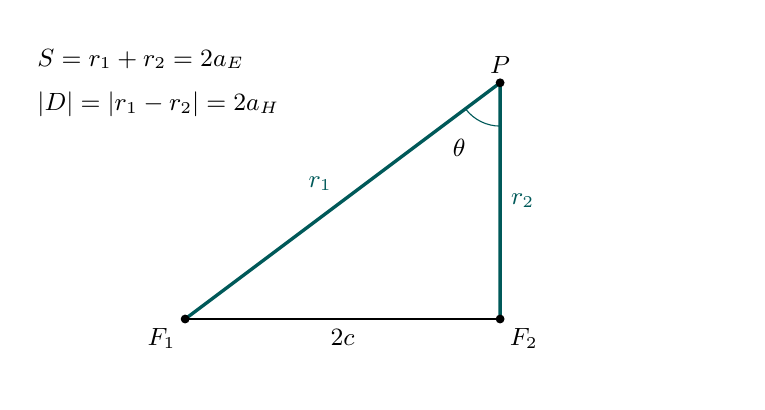
\begin{tikzpicture}[x=1cm,y=1cm,every node/.style={font=\small}]
\path[use as bounding box] (-4,-.8) rectangle (5,3.7);
\coordinate (L) at (-2,0); \coordinate (R) at (2,0); \coordinate (P) at (2,3);
\draw[very thick,teal!70!black] (L)--node[above left] {$r_1$} (P)--node[right] {$r_2$} (R);
\draw[thick] (L)--node[below] {$2c$} (R);
\draw[teal!70!black] (2,2.45) arc(-90:-143.130102:.55);
\node at (1.48,2.18) {$\theta$};
\foreach \v/\lab/\pos in {L/F_1/below left,R/F_2/below right,P/P/above}
  \fill (\v) circle(1.6pt) node[\pos] {$\lab$};
\node[align=left,anchor=west] at (-4,3) {$S=r_1+r_2=2a_E$\\[5pt] $|D|=|r_1-r_2|=2a_H$};
\end{tikzpicture}

\end{center}
\textbf{读图提醒：}如果图形恰画成直角三角形，那只是等号例子的特殊姿态；
此处余弦定理适用于任意 $0<\theta<\pi$ 的非退化焦点三角形。
\textbf{第1步。}对 $\triangle F_1PF_2$ 用余弦定理：
\[
 4c^2=r_1^2+r_2^2-2r_1r_2\cos\theta.
\]
\textbf{第2步。}为什么引入和 $S$、差 $D$？因为椭圆、双曲线的定义恰好
分别提供 $S$ 与 $D^2$，并不直接提供 $r_1^2+r_2^2$ 或 $r_1r_2$。
把 $(r_1\pm r_2)^2$ 展开：
\[
S^2+D^2=2(r_1^2+r_2^2),\qquad
S^2-D^2=4r_1r_2.
\]
所以 $r_1^2+r_2^2=(S^2+D^2)/2$、
$2r_1r_2=(S^2-D^2)/2$，从而
\[
 8c^2=S^2(1-\cos\theta)+D^2(1+\cos\theta).
\]
\textbf{第3步。}代入 $S^2=4c^2/e_1^2$、$D^2=4c^2/e_2^2$，
两边约去 $4c^2$，即
\[
 \boxed{\frac{1-\cos\theta}{e_1^2}+
 \frac{1+\cos\theta}{e_2^2}=2}.
\]
再利用 $1-\cos\theta=2\sin^2(\theta/2)$、
$1+\cos\theta=2\cos^2(\theta/2)$ 得半角形式。
\end{proofbox}

\clearpage
\begin{proofbox}
\textbf{方法二：最低门槛【$A\pm T$，不用额外解未知数】。}


\begin{center}
\begin{tikzpicture}[x=1cm,y=1cm,every node/.style={font=\small}]
\path[use as bounding box] (-1.5,-.7) rectangle (10,3.4);
\node[anchor=west] at (-1.3,3) {右支代表：$a_E=4,\ a_H=1$（同尺度长度图）};
\draw[very thick,blue!70!black] (0,2)--(4,2);
\draw[very thick,red!70!black] (4,2)--(5,2);
\draw[very thick,blue!70!black] (0,.6)--(3,.6);
\draw[dashed,red!70!black,thick] (3,.6)--(4,.6);
\foreach \x/\y in {0/2,4/2,5/2,0/.6,3/.6,4/.6} \draw (\x,\y-.12)--(\x,\y+.12);
\node[above] at (2,2) {$a_E$}; \node[above] at (4.5,2) {$a_H$};
\node[below] at (1.5,.6) {$a_E-a_H$}; \node[below] at (3.5,.6) {$a_H$};
\node[anchor=west] at (5.6,2) {$PF_1=a_E+a_H=5$};
\node[anchor=west] at (5.6,.6) {$PF_2=a_E-a_H=3$};
\node[anchor=west] at (-1.3,-.5) {两条长度之和 $=2a_E$；较长边减较短边 $=2a_H$。};
\end{tikzpicture}

\end{center}
取右支交点，此时 $r_1>r_2$。定义给出
\[
\begin{cases}
r_1+r_2=2a_E &\text{（椭圆：两腰之和固定）},\\
r_1-r_2=2a_H &\text{（双曲线：两腰之差固定）}.
\end{cases}
\]
\textbf{两式相加}消去 $r_2$，$r_1=a_E+a_H$；
\textbf{两式相减}消去 $r_1$，$r_2=a_E-a_H$：
\[
\boxed{r_1=a_E+a_H,\quad r_2=a_E-a_H}\qquad(a_E>c>a_H>0).
\]
$ a_E$ 是\emph{平均长度}，$a_H$ 是\emph{离开平均长度的偏差}。
因为已知两腰、夹角 $\theta$，要求底边 $2c$，所以使用余弦定理：
\[
 \begin{aligned}
 4c^2
 &= (a_E+a_H)^2+(a_E-a_H)^2
   -2(a_E+a_H)(a_E-a_H)\cos\theta\\
 &=2a_E^2(1-\cos\theta)+2a_H^2(1+\cos\theta).
 \end{aligned}
\]
\textbf{为何能化成半角？}由 $1-\cos\theta=2\sin^2(\theta/2)$、
$1+\cos\theta=2\cos^2(\theta/2)$，上式等价于
\[
c^2=a_E^2\sin^2\frac\theta2+a_H^2\cos^2\frac\theta2.
\]
它的几何意义是：$c^2$ 是 $a_E^2,a_H^2$ 的\emph{加权平均}。
两边除以 $c^2$，并代入 $a_E/c=1/e_1$、$a_H/c=1/e_2$ 即得主结论。

\textbf{左支为何不必另证？}左支仅交换两条焦半径的位置，
$\,r_1^2+r_2^2$ 和 $r_1r_2$ 均不变，所以余弦定理结果不变。
\end{proofbox}

\clearpage
\begin{proofbox}
\textbf{方法三：常规解析几何【联立两圆锥曲线方程，复核公共点】。}


\begin{center}
% E: x^2/16+y^2/12=1; H: x^2-y^2/3=1.
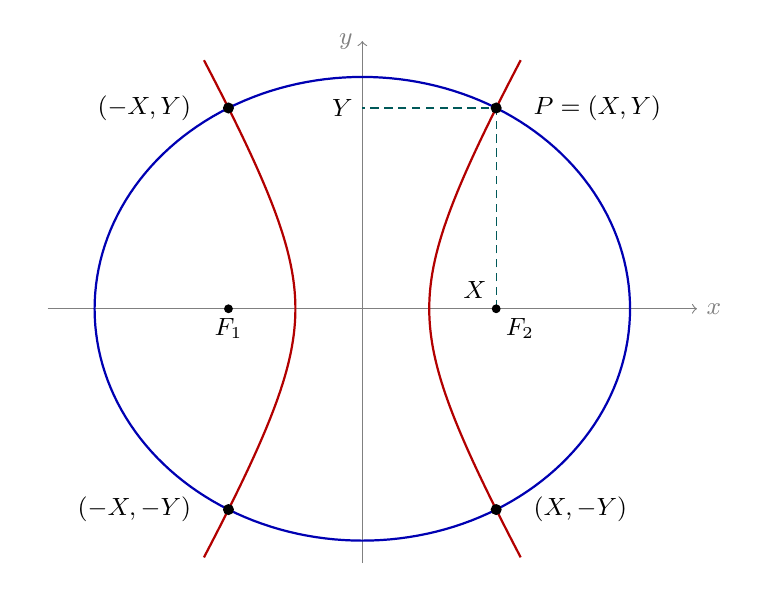
\begin{tikzpicture}[x=.85cm,y=.85cm,every node/.style={font=\small}]
\path[use as bounding box] (-5,-4.1) rectangle (5.8,4.2);
\draw[->,gray] (-4.7,0)--(5,0) node[right] {$x$};
\draw[->,gray] (0,-3.8)--(0,4) node[left] {$y$};
\draw[blue!70!black,thick,domain=0:360,samples=181,variable=\t] plot ({4*cos(\t)},{sqrt(12)*sin(\t)});
\foreach \sgn in {-1,1} \draw[red!70!black,thick,domain=-65:65,samples=121,variable=\t] plot ({\sgn/cos(\t)},{sqrt(3)*tan(\t)});
\draw[densely dashed,teal!70!black] (2,0)--(2,3)--(0,3);
\foreach \x in {-2,2} \foreach \y in {-3,3} \fill (\x,\y) circle(2pt);
\node[right,xshift=10pt] at (2,3) {$P=(X,Y)$};
\node[left,xshift=-10pt] at (-2,3) {$(-X,Y)$};
\node[left,xshift=-10pt] at (-2,-3) {$(-X,-Y)$};
\node[right,xshift=10pt] at (2,-3) {$(X,-Y)$};
\fill (-2,0) circle(1.6pt) node[below] {$F_1$};
\fill (2,0) circle(1.6pt) node[below right] {$F_2$};
\node[above left] at (2,0) {$X$}; \node[left] at (0,3) {$Y$};
\end{tikzpicture}

\end{center}
图中以 $a_E=4,a_H=1,c=2$ 展示四个交点，$X,Y$ 为右上交点的正坐标。

取焦点 $F_1=(-c,0)$、$F_2=(c,0)$，则标准方程为
\[
 E:\ \frac{x^2}{a_E^2}+\frac{y^2}{a_E^2-c^2}=1,
 \qquad H:\ \frac{x^2}{a_H^2}-\frac{y^2}{c^2-a_H^2}=1.
\]
其中 $a_E>c>a_H>0$。
\textbf{为什么可以消元？}两条方程虽然是二次的，却都只出现 $x^2,y^2$，
所以可以把 $x^2,y^2$ 暂看成两个未知数，像初中解二元方程组一样处理。
先分别把 $y^2$ 单独写出来：
\[
\begin{aligned}
y^2&=(a_E^2-c^2)\left(1-\frac{x^2}{a_E^2}\right),\\
y^2&=(c^2-a_H^2)\left(\frac{x^2}{a_H^2}-1\right).
\end{aligned}
\]
令两式右侧相等，移项、合并 $x^2$：
\[
\begin{aligned}
a_E^2-a_H^2
&=x^2\left(\frac{a_E^2-c^2}{a_E^2}
              +\frac{c^2-a_H^2}{a_H^2}\right)\\
&=c^2x^2\left(\frac1{a_H^2}-\frac1{a_E^2}\right)\\
&=\frac{c^2x^2(a_E^2-a_H^2)}{a_E^2a_H^2}.
\end{aligned}
\]
因为 $a_E>a_H$，两边可约去正数 $a_E^2-a_H^2$：
\[
\boxed{x^2=\frac{a_E^2a_H^2}{c^2}}.
\]
回代任意一条曲线方程：
\[
\begin{aligned}
y^2&=(a_E^2-c^2)\left(1-\frac{a_H^2}{c^2}\right)\\
&=\boxed{\frac{(a_E^2-c^2)(c^2-a_H^2)}{c^2}}.
\end{aligned}
\]
\textbf{几何对应：}此时 $x^2>0,y^2>0$，四种正负号给出四个实际交点。
因此 $x\ne0,y\ne0$，四个交点关于两条坐标轴对称，
也证实焦点张角非退化。

任选右上交点 $x=a_Ea_H/c$、$y>0$。
把这两个坐标平方相加，得 $x^2+y^2=a_E^2+a_H^2-c^2$。
为什么要计算 $x^2+y^2$？因为焦半径的平方是
$PF_1^2=(x+c)^2+y^2=x^2+y^2+2cx+c^2$，
$PF_2^2=(x-c)^2+y^2=x^2+y^2-2cx+c^2$，即
\[
 \begin{aligned}
 PF_1^2&=(x+c)^2+y^2=(a_E+a_H)^2,\\
 PF_2^2&=(x-c)^2+y^2=(a_E-a_H)^2.
 \end{aligned}
\]
因 $a_E>a_H>0$，故 $PF_1=a_E+a_H$、$PF_2=a_E-a_H$。
对 $\triangle F_1PF_2$ 用余弦定理，就得到与方法二完全相同的主结论。

\textbf{这法的独立价值：}能直接求四个公共点，核查几何条件确有解，
并可以研究给定标准方程时的具体坐标；若只求主公式，它比前两法繁琐。
\end{proofbox}

\clearpage
\begin{proofbox}
\textbf{推论方法一：最低门槛【平方非负，先理解上界从哪里来】。}

记 $\alpha=\theta/2$，$s=\sin\alpha>0$、$t=\cos\alpha>0$，
并令 $u=1/e_1>0$、$v=1/e_2>0$。主结论变为
\[
 s^2u^2+t^2v^2=1.
\]
\textbf{为什么希望凑出 $st(u+v)$？}目标是 $u+v$，
而 $\sin\theta=2st$，因此只需证明 $st(u+v)\le1$。
再令 $\mathbf q=(su,tv)$、$\mathbf n=(t,s)$、$\mathbf w=(-s,t)$，
后二者为单位正交基，图中以 $\theta=60^\circ,e_1=0.9$ 为代表。

\begin{center}
% Same q as projection figure; orthonormal basis n=(t,s), w=(-s,t).
\begin{tikzpicture}[x=5cm,y=5cm,>=stealth,every node/.style={font=\small}]
\path[use as bounding box] (-.2,-.27) rectangle (2.1,.95);
\pgfmathsetmacro{\k}{sqrt(3)/2*5/9+sqrt(56)/18}
\pgfmathsetmacro{\h}{-5/18+sqrt(3)*sqrt(56)/18}
\coordinate (O) at (0,0); \coordinate (K) at (\k,0); \coordinate (Q) at (\k,\h);
\draw[->,gray] (O)--(1.12,0) node[below] {$\mathbf n$};
\draw[->,gray] (O)--(0,.8) node[left] {$\mathbf w$};
\draw[very thick,teal!70!black] (O)--node[above left] {$1$} (Q);
\draw[very thick,blue!70!black] (O)--node[below] {$k=st(u+v)$} (K);
\draw[very thick,red!70!black] (K)--(Q);
\draw (\k-.06,0)--(\k-.06,.06)--(\k,.06);
\fill (Q) circle(.4pt) node[above] {$\mathbf q$};
\node[anchor=west,align=left] at (1.2,.5) {$h=t^2v-s^2u$\\[7pt] $1-k^2=h^2\ge0$\\[7pt] 等号：高 $h=0$};
\node[anchor=west] at (0,.9) {以单位正交基 $\mathbf n,\mathbf w$ 观察同一向量};
\end{tikzpicture}

\end{center}
\textbf{先用代数，不必先掌握向量：}因为平方必非负，
把目标差式展开，可以直接验证
\[
 (s^2u^2+t^2v^2)-s^2t^2(u+v)^2
   =(s^2u-t^2v)^2\ge0.
\]
所以 $s^2t^2(u+v)^2\le s^2u^2+t^2v^2=1$。
因为 $st>0$，开平方并除以 $st$，得到
\[
\boxed{u+v\le\frac1{st}=\frac2{\sin\theta}}.
\]
\textbf{几何对应：}向量 $\mathbf q=(su,tv)$ 的长度为 $1$，
它在单位方向 $\mathbf n=(t,s)$ 上的投影是 $st(u+v)$，
投影的绝对值不能超过原向量长度 $1$。
差式 $(s^2u-t^2v)^2$ 就是垂直方向投影长度的平方。
等号当且仅当 $s^2u=t^2v$，即垂直方向的投影为 $0$。

\textbf{等号继续推：}等号时 $s^2u=t^2v$，结合 $s^2u^2+t^2v^2=1$
可得 $su=t,tv=s$（均为正），于是
$u=t/s,v=s/t$，也就是 $e_1=s/t=\tan(\theta/2)$、
$e_2=t/s=\cot(\theta/2)$。
\textbf{适用理由：}这个证明不要求先记柯西的配对方法，
而是通过\emph{平方非负}显露出精确的非负余量。
\end{proofbox}

\clearpage
\begin{proofbox}
\textbf{推论方法二：最快证明【柯西--施瓦茨＋等号条件】。}

记 $\alpha=\theta/2\in(0,\pi/2)$，$s=\sin\alpha>0$、
$t=\cos\alpha>0$。主结论化为
\[
 \left(\frac{s}{e_1}\right)^2+
 \left(\frac{t}{e_2}\right)^2=1.
\]
再记 $u=1/e_1,v=1/e_2$。
\textbf{如何想到柯西配对？}目标是 $u+v$，
把它写为 $(su)\cdot(1/s)+(tv)\cdot(1/t)$，
第一组的平方和恰好等于 $1$；第二组平方和由 $s^2+t^2=1$ 化简。
图中 $\mathbf n=st(1/s,1/t)=(t,s)$ 是单位向量。

\begin{center}
% alpha=30 deg, e1=.9; q=(5/9,sqrt(56)/9), |q|=1.
\begin{tikzpicture}[x=4.3cm,y=4.3cm,>=stealth,every node/.style={font=\small}]
\path[use as bounding box] (-.35,-.25) rectangle (2.25,1.15);
\coordinate (O) at (0,0); \coordinate (Q) at ({5/9},{sqrt(56)/9});
\pgfmathsetmacro{\k}{sqrt(3)/2*5/9+sqrt(56)/18}
\coordinate (K) at ({\k*sqrt(3)/2},{\k/2});
\draw[->,gray] (O)--(1.15,0); \draw[->,gray] (O)--(0,1.12);
\draw[gray,dotted,domain=0:90,samples=61] plot ({cos(\x)},{sin(\x)});
\draw[->,very thick,teal!70!black] (O)--(Q) node[above right] {$\mathbf q=(s/e_1,t/e_2)$};
\draw[->,thick,blue!70!black] (O)--({sqrt(3)/2},.5) node[right] {$\mathbf n=(t,s)$};
\draw[red!70!black,dashed,thick] (Q)--(K);
\draw[red!70!black,very thick] (O)--(K);
\node[below right] at (.36,.18) {$k=st(u+v)$};
\node[anchor=west,align=left] at (1.22,.85) {$|\mathbf q|=|\mathbf n|=1$\\[7pt] $k=\mathbf q\cdot\mathbf n\le1$\\[7pt] 等号：两箭头重合};
\node[below] at (0,0) {$O$};
\end{tikzpicture}

\end{center}
投影长度不超过单位向量的长度，代数上即
\[
 \begin{aligned}
 \frac1{e_1}+\frac1{e_2}
 &=\frac{s}{e_1}\cdot\frac1s+
   \frac{t}{e_2}\cdot\frac1t\\
 &\le\sqrt{\frac{s^2}{e_1^2}+\frac{t^2}{e_2^2}}
 \sqrt{\frac1{s^2}+\frac1{t^2}}\\
 &=\frac1{st}=\frac2{\sin\theta}.
 \end{aligned}
\]
\textbf{等号从“向量平行”到具体离心率：}两个正向量
$(s/e_1,t/e_2)$ 与 $(1/s,1/t)$ 成正比例时取等号，
即 $s^2/e_1=t^2/e_2$。
因为 $(s/e_1,t/e_2)$ 是单位向量，且
$(t,s)$ 也是单位向量，等号又意味着它们方向相同，故两者实际上相等：
$s/e_1=t$、$t/e_2=s$。于是
\[
 \frac1{e_1}=\frac{t}{s},\qquad
 \frac1{e_2}=\frac{s}{t},\qquad
 \boxed{e_1=\tan\alpha,\quad e_2=\cot\alpha}.
\]
从 $e_1<1<e_2$ 可知只有 $\alpha<\pi/4$，即 $\theta<\pi/2$，
才可能取等号。反之，对 $0<\theta<\pi/2$ 取
$e_1=\tan(\theta/2)$、$e_2=\cot(\theta/2)$，
主公式成立且由共焦标准方程可以构造公共点，所以等号确实可取。
\end{proofbox}
